\section{Panel Data in the Marketing Analytics Ecosystem}
\label{sec:marketing-ecosystem}

Marketing organisations measure effectiveness through four broad approaches, each with distinct strengths and limitations. Understanding where panel methods fit is essential for choosing the right tool.

Attribution modelling is ubiquitous in digital marketing, but as noted in Section~\ref{sec:measurement-crisis} it remains observational and platform-specific. It reports which touchpoints precede conversions rather than counterfactuals, and often omits spillovers. We use it for optimisation, not for causal effects.

Marketing mix modelling (MMM) can be estimated on aggregate time series or on panels with adstock and saturation. As discussed earlier, aggregate time-series MMM faces identification and spillover challenges and struggles with discrete interventions. Panel MMMs are complementary; our contrast here is with the common aggregate implementation.

The third pillar, geo-experiments, represents the gold standard of causal inference. By randomising treatment across geographic markets -- designated market areas, stores, regions -- firms can generate clean variation in marketing actions that is, by design, uncorrelated with potential outcomes. Geo-experiments are particularly valuable when spillovers are localised within markets (and thus internal to treatment or control clusters) and when the intervention can be implemented at a market level. Platforms including Facebook, Google, and Amazon now offer tools for running geo-experiments at scale, lowering the barrier to adoption. Nevertheless, geo-experiments face practical limitations: spillovers across treatment and control geographies can contaminate estimates, small numbers of geographic clusters limit statistical power, short experimental durations may miss long-run effects, and the cost and complexity of implementing randomised rollouts can be prohibitive.

Panel data methods constitute the fourth pillar. The modern approaches that are the focus of this book apply quasi-experimental identification strategies to observational data, exploiting natural variation in the timing, location, or intensity of marketing actions to estimate causal effects. Unlike attribution models, panel methods explicitly model counterfactual outcomes under control conditions and make testable assumptions about the absence of unobserved confounding. Unlike typical aggregate time-series MMM implementations, panel methods readily isolate discrete interventions, accommodate staggered adoption, and flexibly incorporate unit and time heterogeneity through fixed effects or factor structures. Unlike geo-experiments, panel methods do not require randomisation, enabling analysis of historical data, long-run effects, and settings where randomisation is infeasible. In practice, MMM and panel designs often overlap (for example, panel MMM with adstock and saturation fitted under a design-based identification strategy).

Panel causal designs require design-specific assumptions, not a one-size-fits-all condition. Some methods — difference-in-differences, event studies, interactive fixed effects (Chapters~\ref{ch:did}, \ref{ch:event}, \ref{ch:factor}, \ref{ch:advanced-matrix}) — rely on some form of parallel evolution across treated and control units. Others — synthetic control and its variants (Chapters~\ref{ch:sc}, \ref{ch:generalized-sc}) — substitute strong pre-treatment fit for parallel trends assumptions. Still others — instrumental variables, regression discontinuity, dynamic panel GMM — require entirely different identifying structures: relevance and exclusion, continuity at a threshold, or moment conditions with specific serial correlation patterns. Throughout, we signpost assumptions and diagnostics in Chapters~\ref{ch:did}--\ref{ch:spillovers} and \ref{ch:inference}.

How should a practitioner decide which tool to use? The data structure drives the choice. Without repeated observations on the same units over time, panel methods are off the table. When repeated observations exist, randomisation remains the gold standard. Experiments provide clean identification, though panel methods still add value by controlling for pre-treatment imbalances, quantifying heterogeneity, and extending short-term experimental results through longer observational follow-up. 

When randomisation is infeasible, the structure of treatment variation guides method selection. Discrete interventions at specific points in time call for difference-in-differences or synthetic control methods (Chapters \ref{ch:did}, \ref{ch:event}, \ref{ch:sc}, \ref{ch:generalized-sc}). Treatments that vary smoothly over time or across units without clear pre-post divides suit factor models and matrix completion methods (Chapter \ref{ch:factor}). Spillovers and interference demand methods that explicitly model network or geographic linkages (Chapter \ref{ch:spillovers}). High-dimensional covariates or heterogeneous treatment effects benefit from machine learning integration (Chapters \ref{ch:ml-nuisance}, \ref{ch:high-dim}).

Figure \ref{fig:ecosystem} visualises these four pillars and their relationships. The overlapping circles represent not competition but complementarity. Where the circles intersect, we find opportunities for triangulation. Randomised experiments can validate panel-based estimates and calibrate parameters for marketing mix models. Panel methods can extend short-run experimental results to longer horizons and provide causal interpretations of platform attribution metrics. Marketing mix models can guide the selection of channels for deeper causal analysis. Attribution models can inform which customer segments or touchpoints warrant experimental or quasi-experimental scrutiny. At the centre, where all four approaches converge, lies the principle of triangulation: multiple methods, each with different assumptions and limitations, can collectively build a more robust case for causality than any single method in isolation. The figure also highlights the distinct timelines over which each method operates -- experiments measure effects over days or weeks, panel methods track outcomes over months or years, marketing mix models aggregate data across weeks or quarters, and attribution models provide real-time feedback. Understanding these complementarities and trade-offs is essential for building a comprehensive measurement strategy.

\begin{figure}[htbp]
\centering
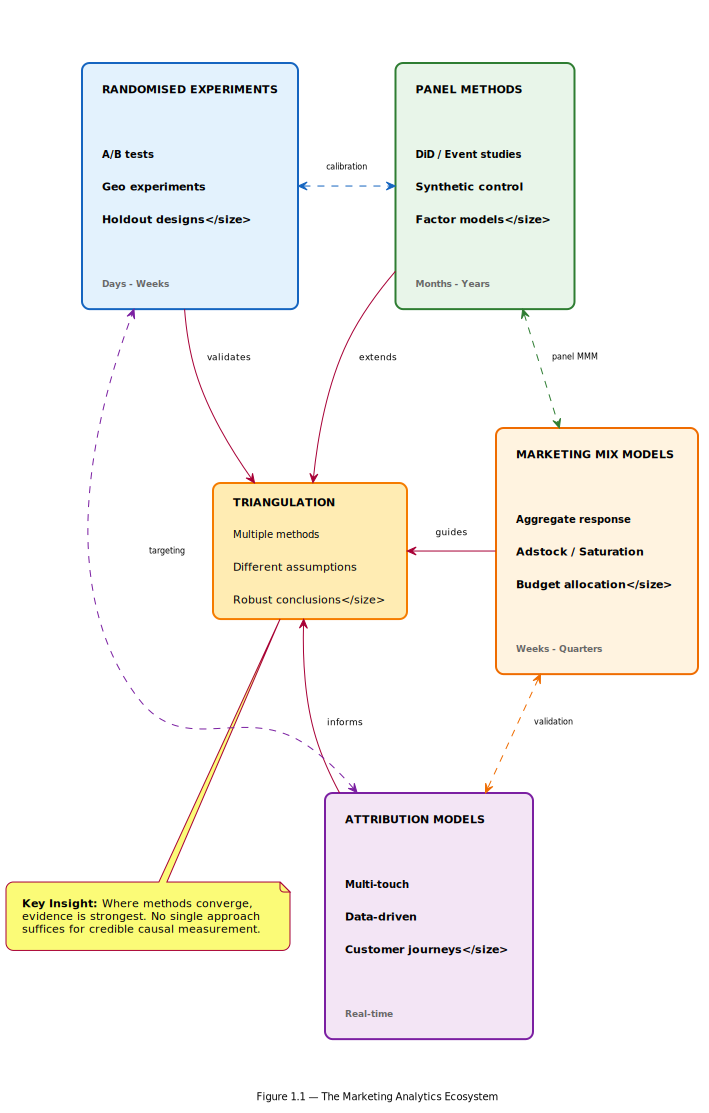
\includegraphics[width=\textwidth]{images/ecosystem.png}
\caption{The Marketing Analytics Ecosystem: Experiments, Panels, MMM, and Attribution}
\label{fig:ecosystem}
\end{figure}

MMM and panel methods are not mutually exclusive. Many workflows combine MMM-style transforms (adstock, saturation) with design-based identification in panels (DiD, SC, IV). Panel MMMs are natural when you have multi-market or store-level data, and design-based logic strengthens identification. Factor-augmented panels (Chapters~\ref{ch:factor}, \ref{ch:advanced-matrix}) and instrumental variables (Chapters~\ref{ch:frameworks}, \ref{ch:inference}) further bridge modelling and design.

Today's methods did not emerge fully formed. They are the product of decades of intellectual development, responding to new data sources, computational capabilities, and substantive challenges. Figure \ref{fig:timeline} traces this evolution from the classical panel econometrics of the 1980s and 1990s -- dominated by two-way fixed effects and random effects models that controlled for time-invariant unobservables -- through the design-based revolution of the 2000s, which brought synthetic control methods and a renewed focus on difference-in-differences with explicit parallel trends assumptions, to the modern era of heterogeneity-robust estimators and machine learning integration. Each wave built on the last, but also responded to limitations exposed by empirical practice. Researchers discovered the negative weighting problem in two-way fixed effects regressions with staggered treatment timing in the late 2010s. This discovery prompted a flurry of new estimators that aggregate cohort-specific treatment effects without using already-treated units as implicit controls. The recognition that parallel trends in levels may be too strong led to synthetic control methods that match on pre-treatment trajectories. The explosion of high-dimensional data -- rich customer covariates, detailed competitor actions, granular geographic and temporal variation -- motivated the integration of machine learning tools for flexible control and heterogeneous effect estimation. This timeline is not just a historical curiosity. It reveals the iterative, self-correcting nature of methodological progress and reminds us that today's cutting-edge methods will themselves be refined, extended, or superseded as new challenges emerge. The marketing applications that drive this book -- loyalty programmes, advertising campaigns, platform expansions -- have been central to this evolution, providing both the motivation for new methods and the empirical testing ground where their strengths and weaknesses become apparent. For a summary of the state of evidence on advertising effectiveness and ROI, see Box 18.5 in Chapter 18, which discusses key findings from Shapiro et al., Blake et al., Gordon et al., Lewis \& Rao, and Erickson \& Jacobson.

\begin{figure}[htbp]
\centering
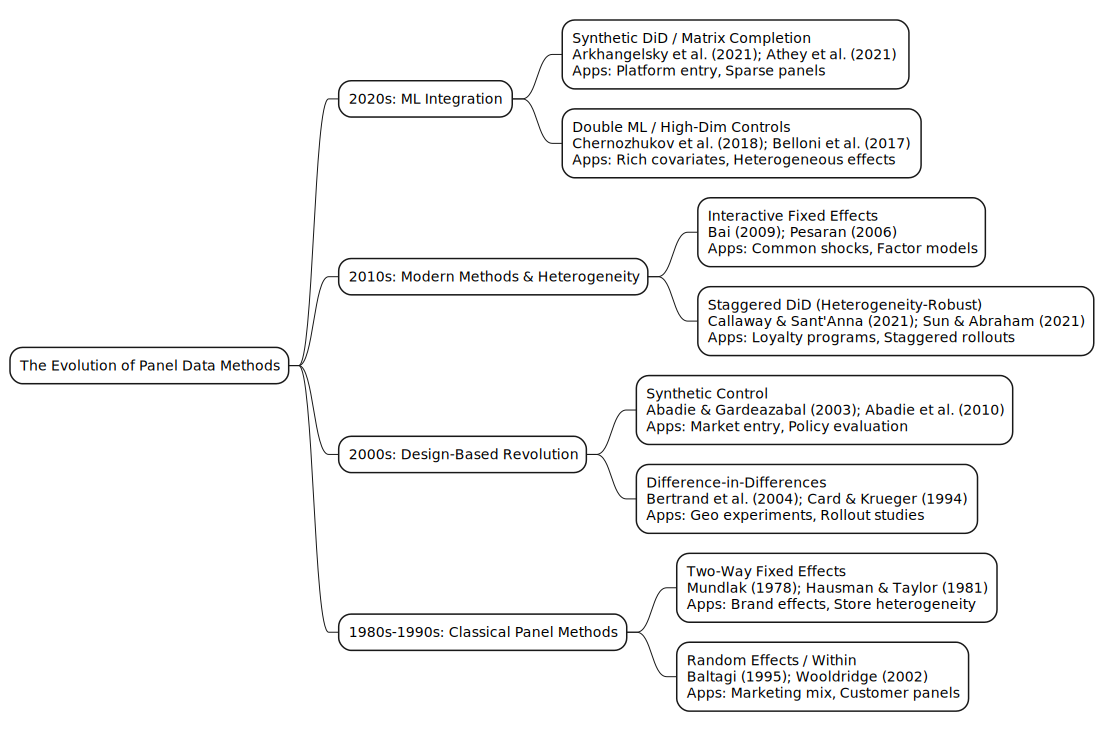
\includegraphics[width=0.8\textwidth]{images/timeline.png}
\caption{Timeline of Panel Data Methods: From TWFE to Modern Heterogeneity-Robust and ML-Integrated Approaches}
\label{fig:timeline}
\end{figure}

The aims of this book grew out of several converging developments rather than a single influence. A sequence of methodological breakthroughs in causal inference for panel data, together with a rapidly expanding applied literature, has made it possible to study marketing interventions with far greater rigour than traditional time-series or attribution approaches allow. At the same time, much of the marketing analytics discourse has drifted toward predictive machine learning, often with only loose connections to identification and design. This book attempts to recentre the discussion on causal structure and research design, while still drawing on modern tools where they genuinely strengthen empirical work.

Within this landscape, the survey by \citet{arkhangelsky2024causal} provides a technically rigorous synthesis of the modern causal panel data literature, covering assignment mechanisms, estimands, difference-in-differences with heterogeneity, synthetic control methods, factor models, and recent advances in inference. We build on much of the same underlying work, but with a different structure and emphasis. First, we prioritise marketing-specific issues — measurement challenges around attribution and platform metrics, threats to validity from seasonality and algorithmic confounding, and substantive applications in loyalty programmes, advertising, pricing, and channel expansion — that receive limited attention in econometrics or finance texts. Second, we integrate recent developments in machine learning for causal inference — double machine learning, causal forests, high-dimensional variable selection — as supporting tools for credible identification rather than as stand-alone prediction technologies. Third, we adopt a practitioner orientation, emphasising intuition, diagnostics, and method selection guidance over formal proofs, while maintaining technical precision in the assumptions and identification arguments.
